\chapter{Geometrie, Information und das Flächengesetz für Schwarze Löcher}

\lectureoverview{Das angekündigte Ziel ist die Kosmologie, doch der kürzeste Weg dorthin beginnt mit einer Rückkehr zur speziellen Relativitätstheorie. Eine Metrik beschreibt die Geometrie der Raumzeit, und die Bedingung verschwindender Eigenzeit beschreibt, wie sich Licht bewegt. Wir übertragen diese eine Regel auf die Schwarzschild-Geometrie, unterscheiden den Horizont von der Singularität und fragen dann, was mit Information geschieht, wenn ein Schwarzes Loch ausstrahlt und verdampft. Die Antwort beginnt mit gewöhnlicher Entropie und endet bei Bekensteins Argument mit einem Bit: Ein Schwarzes Loch speichert Information in Einheiten der Horizontfläche, nicht des Volumens.}

Susskind verschiebt kurz eine angekündigte Bilanz der Erfolge und Misserfolge der Stringtheorie. Es sei spät, sagt er, und die inhaltliche Substanz sei nützlicher als eine Bilanz. Heute Abend geht es um die minimale Geometrie und Thermodynamik, die nötig sind, um das Informationsproblem Schwarzer Löcher zu formulieren.

\section{Eine Regel für Licht}

Die spezielle Relativitätstheorie behandelt Raum und Zeit als ein gemeinsames geometrisches Objekt. Für benachbarte Ereignisse mit dem Abstand \(dt,dx,dy,dz\) verwendet Susskind die Vorzeichenkonvention mit überwiegend positiven Vorzeichen und schreibt
\begin{equation}
d\tau^2=dt^2-\frac{1}{c^2}\left(dx^2+dy^2+dz^2\right).
\end{equation}
Die entgegengesetzten Vorzeichen der zeitlichen und räumlichen Anteile unterscheiden die Minkowski-Geometrie von der vierdimensionalen euklidischen Geometrie. Der Faktor \(1/c^2\) dient lediglich dem Ausgleich der Einheiten; wenn wir Zeit und Entfernung miteinander verträglich messen, können wir \(c=1\) setzen.

Für zeitartige Abstände gilt \(d\tau^2>0\), und \(d\tau\) ist die Eigenzeit, die eine Uhr entlang der Bahn aufzeichnet. Bei raumartigen Abständen gilt dagegen \(d\tau^2<0\). Der heute Abend benötigte Fall liegt genau dazwischen. Ein Lichtstrahl folgt einer \emph{lichtartigen} Bahn,
\begin{equation}
d\tau^2=0.
\end{equation}
Beschränken wir uns zunächst auf eine Bewegung entlang der \(x\)-Achse, so ergibt sich
\begin{align}
0&=dt^2-\frac{dx^2}{c^2},\\
c\,dt&=\pm dx,\\
\frac{dx}{dt}&=\pm c.
\end{align}
Die Vorzeichen beschreiben nach rechts und nach links laufende Strahlen. Der Zahlenwert, der \(c\) zugeordnet wird, ändert sich, wenn Zentimeter durch Meter oder Kilometer ersetzt werden; die invariante Aussage ist keine Zahl, sondern die Nullbedingung.

Die allgemeine Relativitätstheorie macht die Metrik komplizierter, nicht aber diese Regel. Mit den Koordinaten \(x^\mu\), \(\mu=0,1,2,3\) gilt
\begin{equation}
ds^2=g_{\mu\nu}(x)\,dx^\mu dx^\nu,
\end{equation}
wobei über wiederholte Indizes summiert wird und die Koeffizienten sich von Punkt zu Punkt ändern können. Um die lokal möglichen Richtungen des Lichts zu bestimmen, setzt man diese quadratische Form gleich null.

\section{Kugelkoordinaten und die Schwarzschild-Metrik}

Ein nichtrotierendes Schwarzes Loch ist kugelsymmetrisch, daher verdecken kartesische Koordinaten die nützliche Struktur. \(r\) bezeichne den radialen Abstand und \(\theta,\phi\) die Richtung auf einer Einheitskugel. Das Linienelement lautet
\begin{equation}
d\Omega^2=d\theta^2+\sin^2\theta\,d\phi^2.
\end{equation}
Auf einer Kugel mit Radius \(r\) tragen Winkelverschiebungen daher \(r^2d\Omega^2\) bei. Die flache Raumzeit lautet in Kugelkoordinaten
\begin{equation}
d\tau^2=dt^2-\left(dr^2+r^2d\Omega^2\right),
\qquad (c=1).
\end{equation}

Susskind leitet die Lösung für das Schwarze Loch nicht aus Einsteins Gleichungen her. Er schreibt sie hin und bittet uns, sie zu betrachten. Die Tafel macht den beabsichtigten Vergleich deutlich.

\begin{figure}[htbp]
\centering
\includegraphics[width=0.86\textwidth]{lecture_02_figure_02.png}
\caption{Flache Raumzeit in Kugelkoordinaten oberhalb der Schwarzschild-Verformung. Der gemeinsame Faktor \(1-2GM/(c^2r)=1-R_s/r\) und die radiale Skizze sind gleichzeitig zu sehen.}
\lectureframe{00:19:12.520}
\end{figure}

Für ein Schwarzes Loch der Masse \(M\) definieren wir den Schwarzschild-Radius
\begin{equation}
R_s=\frac{2GM}{c^2}.
\end{equation}
Das Linienelement außerhalb des Lochs lautet
\begin{equation}
d\tau^2=\left(1-\frac{R_s}{r}\right)dt^2
-\frac{dr^2/c^2}{1-R_s/r}
-\frac{r^2}{c^2}d\Omega^2.
\label{eq:schwarzschild-explicit-c}
\end{equation}
Äquivalent dazu gilt nach der Setzung \(c=1\)
\begin{equation}
ds^2=\left(1-\frac{2GM}{r}\right)dt^2
-\frac{dr^2}{1-2GM/r}-r^2d\Omega^2.
\label{eq:schwarzschild}
\end{equation}
In großer Entfernung gilt \(R_s/r\ll1\), und die flache Metrik in Kugelkoordinaten ergibt sich zurück. Diese asymptotische Überprüfung ist wichtiger, als die Formel auswendig zu lernen, obwohl Susskind Letzteres als Stoff für Cocktailpartys empfiehlt.

\editorialnote{Auf der Tafel wechseln sich \(d\tau^2\) und \(ds^2\) ab, und nicht jeder Faktor \(c\) wird durchgängig angegeben. Gleichung~\eqref{eq:schwarzschild-explicit-c} folgt der Zeitkoordinatenkonvention der Vorlesung, nach der \(t\) die Einheit einer Zeit hat. Die Standardform mit \(x^0=ct\) ist algebraisch äquivalent.}

\subsection{Der Horizont ist nicht die Singularität}

Bei zwei Radien wirken die Koordinaten verdächtig. Bei \(r=R_s=2GM\) in natürlichen Einheiten verschwindet der Koeffizient von \(dt^2\), während der von \(dr^2\) divergiert. Bei \(r=0\) wird die Krümmung selbst singulär. Das sind keine zwei Varianten desselben Ereignisses:
\begin{equation}
\begin{aligned}
r=R_s &:\quad \text{horizon},\\
r=0 &:\quad \text{curvature singularity}.
\end{aligned}
\end{equation}

Gezeitenkräfte machen den physikalischen Unterschied deutlich. Ein Gravitationsfeld ist über einen ausgedehnten Körper hinweg unterschiedlich: Die Füße können stärker als der Kopf angezogen werden, wodurch der Körper gedehnt und zugleich in Querrichtung zusammengedrückt wird. Am Horizont sind diese Gezeitenkräfte endlich; am Horizont eines hinreichend massereichen Schwarzen Lochs können sie sehr klein sein. Dort muss sich nichts lokal Katastrophales ereignen. Bei \(r=0\) divergieren die Gezeitenkräfte dagegen. Die alarmierenden Koeffizienten bei \(r=R_s\) weisen auf einen Mangel der Schwarzschild-Koordinaten hin; die Singularität bei \(r=0\) ist physikalisch.

\editorialnote{Dass die Krümmung bei \(r=R_s\) endlich ist, lässt sich am Kretschmann-Skalar \(R_{\mu\nu\rho\sigma}R^{\mu\nu\rho\sigma}=48G^2M^2/(c^4r^6)\) überprüfen, der am Horizont endlich ist und nur für \(r\to0\) divergiert. Diese Invariante kam in der Vorlesung nicht vor, präzisiert aber den dort erläuterten Unterschied bei den Gezeitenkräften.}

\section{Radiales Licht in Horizontnähe}

Kehren wir nun zu der einen Regel zurück. Ein radialer Strahl behält seine Winkelposition bei, also gilt \(d\Omega=0\), und für einen Lichtstrahl gilt \(ds^2=0\). In Einheiten mit \(c=1\) ergibt Gleichung~\eqref{eq:schwarzschild}
\begin{equation}
0=\left(1-\frac{2GM}{r}\right)dt^2
-\frac{dr^2}{1-2GM/r}.
\end{equation}
Multiplikation mit \(1-2GM/r\) und anschließendes Wurzelziehen liefern zwei Zweige,
\begin{align}
dr&=\pm\left(1-\frac{2GM}{r}\right)dt,\\
\frac{dr}{dt}&=\pm\left(1-\frac{2GM}{r}\right).
\label{eq:radial-null}
\end{align}
Das Pluszeichen steht für auslaufendes, das Minuszeichen für einlaufendes Licht. In großer Entfernung nähern sich ihre Koordinatengeschwindigkeiten \(\pm1\). Am Horizont gilt für beide \(\lvert dr/dt\rvert\to0\): In Schwarzschild-Koordinatenzeit scheint ein auslaufender Strahl dort stillzustehen, während ein einlaufender Strahl unendlich viel Koordinatenzeit bis zu seiner Ankunft benötigt.

\begin{figure}[htbp]
\centering
\includegraphics[width=0.82\textwidth]{lecture_02_figure_03.png}
\caption{Die vervollständigte Tafelzeichnung im \(t\)-\(r\)-Diagramm: Radiale Nullstrahlen verlaufen nahezu senkrecht, wenn sie sich dem gestrichelten Horizont nähern.}
\lectureframe{00:30:25.000}
\end{figure}

\begin{figure}[htbp]
\centering
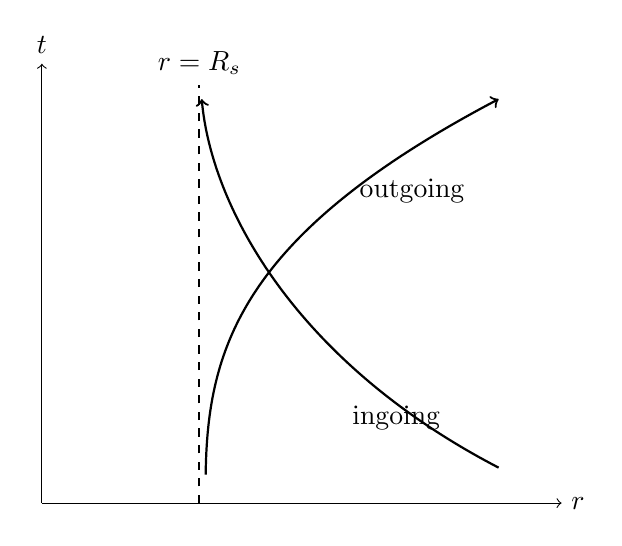
\begin{tikzpicture}[x=1.0cm,y=0.9cm]
\draw[->] (0,0) -- (6.6,0) node[right] {$r$};
\draw[->] (0,0) -- (0,6.2) node[above] {$t$};
\draw[dashed,thick] (2.0,0) -- (2.0,5.9) node[above] {$r=R_s$};
\draw[thick,->] (2.08,.4) .. controls (2.10,2.2) and (2.55,3.8) .. (5.8,5.7);
\draw[thick,->] (5.8,.5) .. controls (3.2,2.0) and (2.15,4.2) .. (2.03,5.7);
\node[align=center] at (4.7,4.4) {outgoing};
\node[align=center] at (4.5,1.2) {ingoing};
\end{tikzpicture}
\caption{Eine bereinigte Fassung der Tafelzeichnung in Koordinatenzeit. Die scheinbare Verlangsamung betrifft \(t\) in Schwarzschild-Koordinaten, nicht ein lokales Versagen des Lichts, sich mit \(c\) zu bewegen.}
\end{figure}

Innerhalb des Horizonts sind die zukünftigen Lichtkegel so weit nach innen geneigt, dass beide zukunftsgerichteten radialen Zweige zu kleinerem \(r\) führen. Kein Signal, das von dort ausgeht, kann nach außen entkommen, und jeder zukunftsgerichtete kausale Weg erreicht die Singularität.

\begin{classroomqa}
\audiencequestion{Wenn die Lichtgeschwindigkeit invariant ist, was genau bedeutet dann die Aussage, dass sich Licht in Horizontnähe verlangsamt?\lecturetimestamp{00:31:44}}
\lecturerresponse{Die dargestellte Größe ist \(dr/dt\) in einem bestimmten Koordinatensystem. Schon die Angabe einer Geschwindigkeit als Zahl ändert sich, wenn Meter durch Zentimeter ersetzt werden; hier variieren die effektiven radialen und zeitlichen Maßstäbe mit dem Ort. Die universelle Aussage lautet, dass jeder Lichtstrahl einer Nullbahn folgt: \(ds^2=0\).}
\end{classroomqa}
\editorialnote{Ein frei fallender lokaler Beobachter misst für Licht im Vakuum \(c\); die verschwindende Schwarzschild-Koordinatengeschwindigkeit am Horizont ist keine lokal beobachtbare Größe.}

\begin{classroomqa}
\audiencequestion{Gilt dieselbe Aussage über die Nullgeschwindigkeit unabhängig vom materiellen Medium, durch das sich das Licht bewegt?\lecturetimestamp{00:33:24}}
\lecturerresponse{Nein. Die verfügbare Aufzeichnung enthält keine längere Erklärung dieser Antwort.}
\end{classroomqa}
\editorialnote{Die Aussage über die Nullgeschwindigkeit betrifft die Ausbreitung in der Vakuumraumzeit. Wechselwirkungen mit Materie können einem Wellenpaket eine geringere effektive Geschwindigkeit verleihen; das ist eine Eigenschaft des Mediums und keine Änderung der lokalen kausalen Geschwindigkeit \(c\).}

\begin{classroomqa}
\audiencequestion{Wie sieht ein einlaufender Lichtstrahl im selben \(t\)-\(r\)-Diagramm aus?\lecturetimestamp{00:33:32}}
\lecturerresponse{Er ist der umgekehrt erscheinende Zweig: Ausgehend von großem \(r\) biegt er zum Horizont hin ab und nähert sich diesem asymptotisch. Bis zur Ankunft vergeht eine unendliche Koordinatenzeit \(t\).}
\end{classroomqa}
\editorialnote{Ein einfallender Beobachter erreicht und durchquert den Horizont in endlicher Eigenzeit; nur die Schwarzschild-Koordinatenzeit \(t\) divergiert.}

\section{Warum die Verdampfung ein Problem aufwirft}

Der Horizont verdient eine viel eingehendere Untersuchung: wie er entsteht, was ein einfallender Beobachter sieht und ob sich dort lokal etwas Ungewöhnliches ereignet. Susskind vertagt diese Fragen und springt zur Quantenmechanik. Von außen betrachtet werden Materie und sämtliche unterscheidenden Informationen immer näher an den Horizont herangedrückt und unzugänglich. Das allein muss keine Information vernichten; sie könnte lediglich verborgen sein.

Hawkings Ergebnis macht das Problem akut. Ein klassisches Schwarzes Loch im Gleichgewicht wirkt wie das langweiligste denkbare Objekt: kugelförmig, dunkel und unfähig, eine Nachricht zu senden. Doch ``schwarz'' hat zwei Bedeutungen. Es kann heißen, dass nichts ausgestrahlt wird, oder dass thermische Schwarzkörperstrahlung ausgesandt wird. Ein quantenmechanisches Schwarzes Loch ist im zweiten Sinn schwarz. Es hat eine Temperatur, leuchtet und verliert Energie. Da
\begin{equation}
E=Mc^2,
\qquad
R_s=\frac{2GM}{c^2},
\end{equation}
verringert die Strahlung sowohl seine Masse als auch seinen Horizont-Radius. Was geschieht mit der Information, die am Horizont verblieben zu sein schien, wenn das Loch schließlich verdampft? Sie könnte vernichtet, in einem winzigen Überrest eingeschlossen oder in der auslaufenden Strahlung kodiert sein. Die Spannung zwischen diesen Möglichkeiten ist das Informationsproblem, und die Stringtheorie wird später helfen, seine Lösung genauer zu fassen.

Heute Abend wird keine Berechnung von Quantenfeldern in gekrümmter Raumzeit vorgenommen. Stattdessen folgt Susskind Bekensteins einfacherer Vorgehensweise: Zuerst verstehen wir Entropie als Information und berechnen dann, wie viel Information ein Schwarzes Loch verbergen kann.

\section{Information, die vorhanden, aber verborgen ist}

Stellen wir uns vor, eine Schachtel werde in Zellen unterteilt, die so klein sind, dass jede entweder belegt oder leer ist. Eine binäre Zeichenfolge---eine Antwort pro Zelle---unterscheidet die jeweilige Konfiguration von jeder anderen zulässigen Konfiguration. Für realistischere Materie muss man auch nach Teilchensorten und weiteren Freiheitsgraden fragen, aber das Prinzip bleibt gleich: Information wird durch die Mindestzahl an Ja--Nein-Fragen gemessen, die nötig ist, um den Zustand festzulegen.

\begin{classroomqa}
\audiencequestion{Beschreibt das nur ein statisches System?\lecturetimestamp{00:45:49}}
\lecturerresponse{Es ist eine Momentaufnahme zu einem bestimmten Zeitpunkt. Die Dynamik bildet diesen Zustand dann auf einen anderen ab.}
\end{classroomqa}

Das nächste Prinzip geht tiefer: Die Entwicklung eines abgeschlossenen Systems führt nicht zwei verschiedene mikroskopische Zustände zu einem einzigen zusammen. Unterscheiden sich zwei Konfigurationen jetzt, bleiben auch ihre entwickelten Konfigurationen prinzipiell unterscheidbar. Die klassische Hamiltonsche Entwicklung ist umkehrbar, die quantenmechanische Entwicklung unitär.\editorialnote{Dissipative effektive Gleichungen können Unterschiede nur deshalb auslöschen, weil unbeobachtete Freiheitsgrade der Umgebung weggelassen wurden; der vollständige Zustand des abgeschlossenen Systems bewahrt sie.}

Die Badewanne macht den Unterschied zwischen Verlust und Unzugänglichkeit anschaulich. Zwei Tropfenströme könnten zwei verschiedene Morsecode-Nachrichten kodieren. Nachdem sich das Wasser beruhigt hat, sehen beide Wannen gleich aus. Die sichtbaren Wellen sind verschwunden, doch eine vollständige mikroskopische Messung würde weiterhin unterschiedliche Molekülkonfigurationen ergeben. Die Nachricht hat sich auf Freiheitsgrade verteilt, die zu klein und zu zahlreich sind, um sie zu verfolgen.

Entropie ist diese verborgene Information. Gemessen an den makroskopischen Fragen, die wir stellen können---Temperatur, Gesamtenergie, Zusammensetzung, Wasserstand---, bleiben viele mikroskopische Unterschiede möglich, aber unzugänglich. In der Bit-Zählweise der Vorlesung gilt
\begin{equation}
S=\hbox{number of hidden bits}.
\end{equation}
Die genaue statistische Formel lautet \(S=k_B\ln\Omega\), doch für das Argument zu Schwarzen Löchern genügt die qualitative Definition.

\section{Temperatur als Preis für das Verbergen eines Bits}

Temperatur lässt sich leicht messen, aber überraschend indirekt definieren. Susskind wählt Entropie und Energie als Grundbegriffe. Angenommen, ein Computerbit wird auf einen Standardwert zurückgesetzt. Das physische Gerät bleibt bestehen, doch der Unterschied zwischen seinem früheren Null- und Einszustand verschwindet im Computer. Aus der vollständigen Welt kann er nicht verschwinden; er wird auf mikroskopische Freiheitsgrade der Umgebung übertragen, die sich dadurch geringfügig erwärmt. Das ist das Landauer-Prinzip.

Wenn eine Entropieeinheit einem Bit entspricht und die Temperatur in Energieeinheiten gemessen wird, schreibt die Vorlesung
\begin{align}
\Delta S&=1,\\
\Delta E&=T\,\Delta S,\\
dE&=T\,dS.
\label{eq:first-law}
\end{align}

\begin{figure}[htbp]
\centering
\includegraphics[width=0.84\textwidth]{lecture_02_figure_04.png}
\caption{Die informationstheoretische Thermodynamik auf der Tafel: \(S\) ist die Entropie, ein verborgenes Bit entspricht \(\Delta S=1\), und sein minimaler Energieaufwand wird mit \(\Delta E=T\Delta S\) angegeben.}
\lectureframe{00:58:40.000}
\end{figure}

\editorialnote{In konventionellen Einheiten beträgt der reversible Löschaufwand für ein binäres Bit \(k_BT\ln2\). Gleichung~\eqref{eq:first-law} verwendet \(k_B=1\) und behandelt die Entropieeinheit der Vorlesung als ein Bit, wobei der zugehörige Faktor \(\ln2\) unterdrückt wird. Diese Konventionen ändern nichts an der folgenden Skalierungsbetrachtung.}

Eine Schätzung aus dem Publikum beziffert den minimalen Temperaturanstieg beim Löschen von etwa \(100\) Gigabyte in einem Glas Wasser auf ungefähr \(10^{-15}\) Grad. Susskind lässt die genaue Zahl dahingestellt und übernimmt den wesentlichen Punkt: Bei Raumtemperatur trägt ein Bit eine außerordentlich kleine minimale Energie, und reale Computer dissipieren erheblich mehr, weil das Löschen nicht reversibel erfolgt.

\begin{classroomqa}
\audiencequestion{Ist das Festplattenbeispiel nur eine Analogie, oder ist die Erwärmung beim Löschen ein echtes Gesetz?\lecturetimestamp{01:00:02}}
\lecturerresponse{Es handelt sich um eine echte physikalische Einschränkung, die Landauer-Regel. Beim Zurücksetzen einer Speicherzelle verschwindet die alte Unterscheidung aus dem Computer, also muss die Information in die Umgebung übertragen werden. Gewöhnliche Vorgänge sind viel weniger effizient als das ideale Minimum, weil sie außerdem Schaltkreise antreiben, Ladungen bewegen und nicht damit zusammenhängende Wärme erzeugen.}
\end{classroomqa}

\begin{classroomqa}
\audiencequestion{Kostet es bei höherer Temperatur mehr Energie, ein Bit zu verbergen?\lecturetimestamp{01:02:07}}
\lecturerresponse{Ja. Die Beziehung \(dE=T\,dS\) besagt genau das: Für dieselbe übertragene Entropie erfordert ein heißeres Wärmebad eine größere Energieübertragung. Ebenso kann man diese Beziehung zwischen Energie und verborgenem Bit als Definition der Temperatur auffassen.}
\end{classroomqa}

\begin{classroomqa}
\audiencequestion{Geht die zuvor gespeicherte Information verloren, wenn man ein Bit überschreibt?\lecturetimestamp{01:02:43}}
\lecturerresponse{Sie hat den Computer verlassen, ist aber nicht aus dem abgeschlossenen physikalischen System verschwunden. Der überschriebene Unterschied hat sich in der Umgebung verteilt, wo er zu unzugänglicher Information und damit zur Entropie beiträgt.}
\end{classroomqa}

Die Gleichsetzung thermodynamischer Entropie mit fehlender mikroskopischer Information geht auf Boltzmann zurück; Shannon entwickelte im zwanzigsten Jahrhundert die entsprechende informationstheoretische Sprache. Susskind merkt an, dass diese Erklärung in den Thermodynamikkursen, die er und einige Zuhörer besucht hatten, merkwürdigerweise fehlte, und zwar in den 1950er-Jahren. Die Informatik machte es schwerer, den Zusammenhang zu übersehen, begründete aber nicht seinen physikalischen Gehalt.

\section{Ein Bit in ein Schwarzes Loch einbringen}

Nun können wir uns gedanklich ein Schwarzes Loch Bit für Bit aufbauen, so wie sich eine Badewanne Tropfen für Tropfen füllen lässt. Die Frage ist eine differentielle: Um wie viel wächst der Horizont, wenn ein weiteres Bit verborgen wird? Wir beginnen mit einem Loch der Masse \(M\) und des Radius \(R_s\) und schicken dann das einfachste Objekt hinein, dessen einzige wiedergewinnbare Unterscheidung darin besteht, ob es absorbiert wurde.

\begin{classroomqa}
\audiencequestion{Benötigt die Information nicht unendlich viel Koordinatenzeit, um in das Loch zu gelangen?\lecturetimestamp{01:08:07}}
\lecturerresponse{In Horizontnähe wird sie exponentiell komprimiert und dem Außenbereich nach kurzer praktischer Zeit unzugänglich, obwohl die Schwarzschild-Koordinatenzeit für die tatsächliche Überquerung einen unendlichen Wert angibt. Für die Bilanz von außen kann man sie daher so behandeln, als sei sie am Horizont gespeichert.}
\end{classroomqa}

Ein Photon ist ein naheliegender Kandidat, trägt aber im Allgemeinen mehr als ein Bit. Seine Polarisation kann eine binäre Wahl kodieren. Ein genau bestimmter Ankunftsort liefert viele weitere Ja--Nein-Fragen: obere oder untere Hemisphäre, linke oder rechte Hälfte und so weiter. Die Quantenmechanik begrenzt die Lokalisierung auf ungefähr eine Wellenlänge; um die Ortsinformation zu unterdrücken, verwendet man daher die längste Wellenlänge, die das Loch noch absorbieren kann.

\begin{classroomqa}
\audiencequestion{Gibt es tatsächlich eine obere Grenze für die Wellenlänge, oberhalb derer das Photon nicht mehr eindringen kann?\lecturetimestamp{01:12:15}}
\lecturerresponse{Ja. Eine Welle, die viel größer als das Loch ist, wird überwiegend gestreut statt absorbiert. Die geeignete Grenzwahl ist eine Wellenlänge in der Größenordnung des Horizont-Radius: lang genug, um den Eintrittsort zu verwischen, und zugleich kurz genug, um eine beträchtliche Absorptionswahrscheinlichkeit zu haben.}
\end{classroomqa}

\begin{classroomqa}
\audiencequestion{Liefert die Richtung, aus der das Photon eintrifft, zusätzliche Information?\lecturetimestamp{01:13:28}}
\lecturerresponse{Bei einer Wellenlänge in der Größenordnung des gesamten Horizonts ändert sich das Feld über das Loch hinweg so langsam, dass sich die Einfallsrichtung nicht mit großer Genauigkeit bestimmen lässt. Deshalb lässt sich der Grenzfall großer Wellenlängen näherungsweise durch ein einzelnes Ja--Nein-Datum beschreiben, statt durch einen genau lokalisierten Einschlag.}
\end{classroomqa}

Wir wählen also größenordnungsmäßig
\begin{equation}
\lambda\sim R_s=\frac{2GM}{c^2}.
\label{eq:one-bit-wave}
\end{equation}
Aus der Kinematik des Photons folgt
\begin{equation}
E=cp,
\qquad
p=\hbar k=\frac{h}{\lambda},
\qquad
\Delta E\sim\frac{\hbar c}{R_s}.
\label{eq:one-bit-energy}
\end{equation}
Dabei gilt \(k=2\pi/\lambda\) und \(h=2\pi\hbar\). In der Vorlesung wird der Faktor \(2\pi\) bewusst vernachlässigt, ebenso wie Faktoren der Absorption in der Größenordnung eins.

\begin{classroomqa}
\audiencequestion{Sollte der Impuls als \(\hbar/\lambda\) oder als \(h/\lambda\) geschrieben werden?\lecturetimestamp{01:16:00}}
\lecturerresponse{Mit \(\lambda\) als gewöhnlicher Wellenlänge lautet die exakte Beziehung \(p=h/\lambda=2\pi\hbar/\lambda\); mit der Wellenzahl \(k=2\pi/\lambda\) lautet sie \(p=\hbar k\). In der vorliegenden Abschätzung behalten wir nur die Größenordnung bei und lassen den Faktor \(2\pi\) bewusst weg.}
\end{classroomqa}

Die Energiekosten für das Verbergen eines Bits legen die Temperaturskala fest. Aus den Gleichungen~\eqref{eq:one-bit-wave} und~\eqref{eq:one-bit-energy} folgt daher
\begin{equation}
k_BT_H\sim\frac{\hbar c}{R_s}
\sim\frac{\hbar c^3}{GM}.
\end{equation}
Das exakte Hawking-Ergebnis lautet
\begin{equation}
k_BT_H=\frac{\hbar c^3}{8\pi GM}.
\end{equation}
Das elementare Argument liefert die Abhängigkeit von \(M,G,c,\hbar\), nicht aber den Koeffizienten.

\section{Ein Bit belegt ein Flächenelement in der Planck-Skala}

Dasselbe Photon verrät uns, wie der Horizont wächst. Seine Energie ändert die Masse um
\begin{equation}
\Delta M=\frac{\Delta E}{c^2}
\sim\frac{\hbar}{cR_s}.
\end{equation}
Da \(R_s=2GM/c^2\) gilt,
\begin{equation}
\Delta R_s=\frac{2G}{c^2}\Delta M
\sim\frac{G\hbar}{c^3R_s},
\end{equation}
wobei erneut alle Faktoren in der Größenordnung eins unterdrückt wurden. Multiplizieren wir mit \(R_s\),
\begin{equation}
R_s\Delta R_s\sim\frac{G\hbar}{c^3}.
\end{equation}
Da \(A=4\pi R_s^2\) gilt, lautet das Differential \(dA=8\pi R_s\,dR_s\). Somit
\begin{equation}
\Delta A\sim\frac{G\hbar}{c^3}=\ell_P^2,
\qquad
\ell_P=\sqrt{\frac{G\hbar}{c^3}}.
\label{eq:planck-patch}
\end{equation}

\begin{figure}[htbp]
\centering
\includegraphics[width=0.84\textwidth]{lecture_02_figure_05.png}
\caption{Die vollständige Skalierungsbetrachtung auf der Tafel: Die Energie für ein Bit \(\Delta E\sim\hbar c/R_s\) führt zu einer Zunahme des Radiusquadrats und damit der Fläche in der Größenordnung von \(G\hbar/c^3\).}
\lectureframe{01:22:40.000}
\end{figure}

Während der Rechnung an der Tafel werden die Faktoren \(c\) mitten in der Rechnung wieder eingesetzt, und ein Zuhörer bemerkt, dass im Schwarzschild-Radius der Faktor \(c^{-2}\) fehlt. Genau diese Korrektur ergibt den Faktor \(c^{-3}\) in Gleichung~\eqref{eq:planck-patch}.

\begin{classroomqa}
\audiencequestion{Gehen durch das Wiedereinsetzen von \(c\) nur in einem Teil der Rechnung zwei Potenzen davon verloren?\lecturetimestamp{01:21:18}}
\lecturerresponse{Ja. Die Dimensionsbeziehung lautet \(R_s=2GM/c^2\) und nicht einfach \(2GM\). Mit diesem Faktor ergibt sich für die Fläche die Skalierung \(G\hbar/c^3\).}
\end{classroomqa}

Mit \(G\simeq6.7\times10^{-11}\,\mathrm{m^3\,kg^{-1}\,s^{-2}}\), \(\hbar\simeq1.05\times10^{-34}\,\mathrm{J\,s}\) und \(c^3\simeq2.7\times10^{25}\,\mathrm{m^3\,s^{-3}}\) gilt
\begin{equation}
\ell_P^2\simeq2.6\times10^{-70}\,\mathrm{m^2},
\qquad
\ell_P\simeq1.6\times10^{-35}\,\mathrm{m}.
\end{equation}
Während der Abschätzung an der Tafel schwanken die verbal genannten Potenzen in der Vorlesung; die physikalische Schlussfolgerung bleibt bestehen. Diese Skala liegt weit unterhalb der direkten experimentellen Auflösung.

Das einprägsame Bild zeigt undurchdringliche Bits mit spitzen Ellbogen, die sich am Horizont ansammeln und gegenseitig verdrängen. Jedes neue Bit beansprucht ungefähr ein Planck-Flächenelement. Das ist eine Metapher für die Flächenbilanz, keine Behauptung, der Horizont bestehe tatsächlich aus quadratischen Kacheln.

\begin{classroomqa}
\audiencequestion{Wenn sich das erste Photon noch nähert, während ein weiteres Photon den Horizont vergrößert, liegt das erste dann nicht innerhalb des neuen Horizonts?\lecturetimestamp{01:26:39}}
\lecturerresponse{Das einfache statische Bild reicht nicht aus, um diese Frage präzise zu beantworten. Der Ereignishorizont einer dynamischen Raumzeit muss global definiert werden, und seine Lage ändert sich, wenn Materie eintrifft. In der hier verwendeten Beschreibung von außen bleibt die Information dem wachsenden Horizont zugeordnet. Eine sorgfältige Definition dieses Horizonts wird auf später verschoben.}
\end{classroomqa}

\begin{classroomqa}
\audiencequestion{Ergäbe sich dasselbe Problem, wenn eine große Masse hinzukäme, etwa bei der Kollision zweier Schwarzer Löcher?\lecturetimestamp{01:27:03}}
\lecturerresponse{Ja; dann lässt sich der dynamische Charakter nicht mehr ignorieren. Die Vorlesung verschiebt die vollständige Geometrie der Verschmelzung, bis der Horizont genauer definiert worden ist.}
\end{classroomqa}

\begin{classroomqa}
\audiencequestion{Ist eine Planck-Fläche nur auf einem flachen Flächenstück definiert und nicht auf einem kugelförmigen Horizont?\lecturetimestamp{01:27:30}}
\lecturerresponse{Sie ist eine Flächenskala auf der Kugeloberfläche; der Horizont muss nicht flach sein. Für diese Zählung ist der Unterschied zwischen eben und kugelförmig unerheblich.}
\end{classroomqa}
\editorialnote{Wenn der Krümmungsradius des Horizonts viel größer als \(\ell_P\) ist, ist jede Umgebung in Planck-Größe lokal nahezu flach.}

Bei einem Schwarzen Loch mit acht Kilometern Durchmesser hat das maßgebliche Photon entsprechend eine lange Radiowellenlänge in etwa dieser Größenordnung. Eine Analogie aus dem Publikum vergleicht die größenunabhängige Flächenzunahme damit, einer um einen Basketball oder um die Erde gewickelten Schnur denselben zusätzlichen Umfang hinzuzufügen: In beiden Fällen ist der dadurch entstehende radiale Abstand gleich. Die genauen Geometrien unterscheiden sich, doch beide Beispiele veranschaulichen eine Änderung, die unabhängig von der ursprünglichen Größe des Objekts ist.

\section{Das Flächengesetz}

Wenn man Bit für Bit hinzufügt, ändert sich die Horizontfläche um einen universellen mikroskopischen Betrag. Die Zahl der Bits, die verborgen werden können, muss daher proportional zu \(A/\ell_P^2\) sein, nicht zum Volumen. Bekenstein erschloss die Proportionalität; Hawking bestimmte ihren Koeffizienten:
\begin{equation}
S_{\mathrm{BH}}=\frac{k_B A c^3}{4G\hbar}
=\frac{k_B A}{4\ell_P^2}.
\label{eq:bh-entropy}
\end{equation}
Wird die Entropie in binären Bits statt in thermodynamischen Einheiten gezählt, teilt man \(S_{\mathrm{BH}}/k_B\) durch \(\ln2\).

\begin{figure}[htbp]
\centering
\includegraphics[width=0.84\textwidth]{lecture_02_figure_06.png}
\caption{Die abschließende Formel auf der Tafel, einschließlich Hawkings Faktor \(1/4\): \(S\propto Ac^3/(4G\hbar)\) in den Entropieeinheiten der Vorlesung.}
\lectureframe{01:31:02.000}
\end{figure}

Schwarze Löcher haben daher erheblich mehr Entropie als gewöhnliche Systeme vergleichbarer Größe. Dennoch ist der Wert kleiner, als eine naive Zählung nach Volumen erwarten ließe. Die unabhängige Information ist durch eine Größe begrenzt, die die Oberfläche misst. Diese Umkehrung---ein dreidimensionaler gravitativer Bereich, beschrieben durch Information, die mit einer zweidimensionalen Begrenzungsfläche skaliert---, ist der Ausgangspunkt des holografischen Prinzips.

\begin{classroomqa}
\audiencequestion{Woher stammt der Faktor \(1/4\) in der Entropieformel?\lecturetimestamp{01:30:30}}
\lecturerresponse{Bekensteins Argument bestimmte die Abhängigkeit von der Fläche und den Fundamentalkonstanten, ließ aber den Koeffizienten offen; seine Abschätzungen ergaben Möglichkeiten wie etwa Zweierlogarithmen. Hawkings quantenfeldtheoretische Berechnung bestimmte den Koeffizienten exakt zu \(1/4\).}
\end{classroomqa}

Die Stellung von \(\hbar\) birgt die letzte Überraschung. Man könnte erwarten, dass eine Quantenentropie proportional zu \(\hbar\) ist und im klassischen Grenzfall verschwindet. Stattdessen steht \(\hbar\) im Nenner. Wenn \(\hbar\to0\), kann eine Welle beliebig feine Information bei beliebig geringen Energiekosten tragen, sodass die Entropiekapazität divergiert. Die Quantisierung fügt einem ansonsten klassischen Loch keine winzige Entropie hinzu; sie verhindert, dass seine Informationskapazität unendlich ist.

\begin{classroomqa}
\audiencequestion{Warum bestimmt \(\hbar\), dessen Einheit der des Drehimpulses entspricht, auch die Beziehung zwischen gewöhnlichem Impuls und Wellenlänge?\lecturetimestamp{01:33:23}}
\lecturerresponse{\(\hbar\) hat die Einheit einer Wirkung, also gleichwertig Impuls mal Länge. Da \(p\lambda\) dieselbe Einheit hat, kann die Quantenbeziehung bis auf die Konvention für \(p\sim\hbar/\lambda\) als \(2\pi\) geschrieben werden. Aus demselben Grund hat auch der Drehimpuls \(\mathbf r\times\mathbf p\) dieselbe Dimension.}
\end{classroomqa}

Die Vorlesung endet hier, nicht weil das Thema erschöpft wäre, sondern weil dies die richtige Grenze ist. Die Geometrie hat uns gezeigt, warum der Horizont Information verbirgt; die Thermodynamik hat uns gezeigt, wie sich verborgene Information zählen lässt; die Quantenmechanik hat eine endliche Fläche pro Bit geliefert. Die nächste Frage lautet nicht mehr, ob ein Schwarzes Loch mikroskopische Zustände besitzt, sondern wie diese Zustände kodieren, was hineingefallen ist, und es schließlich zurückgeben.